\documentclass{article}
\usepackage[T1]{fontenc}
\usepackage{lmodern}
\usepackage{graphicx}
\usepackage{amsmath,amssymb}
\usepackage[a4paper,margin=2cm]{geometry}
\usepackage[absolute,overlay]{textpos}
\setlength{\TPHorizModule}{1mm}
\setlength{\TPVertModule}{1mm}
\usepackage[indonesian]{babel}
\usepackage{hyperref}
\setlength{\emergencystretch}{2em}
% unit: Halaman 32

\begin{document}

% === Halaman 32 (llm) ===

4. Kalikan vektor kolom bit $(b_0, b_1, ..., b_8)^T$ dengan sebuah matriks \textit{affine} sebagai berikut:

\vspace{10mm}

5. Selanjutnya, konversi hasil perhitungan $(b'_0, b'_1, ..., b'_8)^T$ ke dalam heksadesimal, menjadi elemen $S\text{-}box(x, y)$.

% deskripsi: Persamaan perkalian matriks affine untuk transformasi bit dalam S-box, melibatkan matriks 8x8, vektor kolom b, dan vektor konstanta dengan operasi XOR.
% bbox normalisasi: [0.1860, 0.2660, 0.6840, 0.7340]
\begin{textblock*}{104.58mm}(39.06mm,79.00mm)
\noindent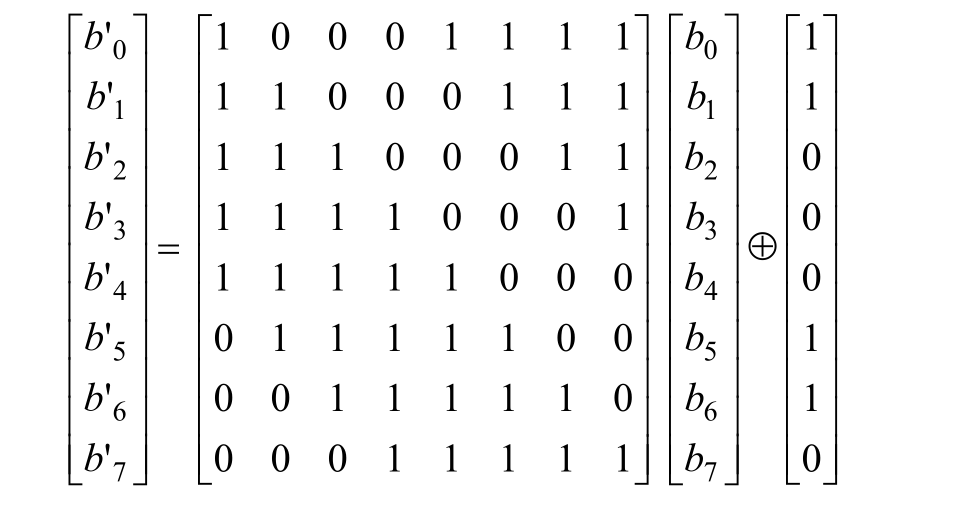
\includegraphics[width=104.58mm,height=139.00mm]{../../images/llm/page_032_img_01.png}%
\end{textblock*}

\end{document}
